\documentclass[10pt]{article}


% This is a helpful package that puts math inside length specifications
%\usepackage[default]{lato}
%\usepackage[T1]{fontenc}
\usepackage{multirow}
\usepackage{wasysym}
\usepackage{marginnote}
\usepackage{url}
\usepackage{calc}
\usepackage[spanish, es-tabla]{babel}
\usepackage[utf8]{inputenc}
\usepackage{graphicx}
\usepackage{xcoffins}
\usepackage{array}
\usepackage{multicol}
\usepackage{multirow}
\usepackage{titlesec}
\usepackage[scaled=.90]{helvet}
\usepackage{fancyhdr}
%\usepackage{markdown}
\usepackage[ddmmyyyy,hhmmss]{datetime}
\titleformat{\section}
  {\normalfont\sffamily\Large\bfseries\color{cyan}}
  {\thesection}{1em}{}

% Layout: Puts the section titles on left side of page
\reversemarginpar

%
%         PAPER SIZE, PAGE NUMBER, AND DOCUMENT LAYOUT NOTES:
%
% The next \usepackage line changes the layout for CV style section
% headings as marginal notes. It also sets up the paper size as either
% letter or A4. By default, letter was used. If A4 paper is desired,
% comment out the letterpaper lines and uncomment the a4paper lines.
%
% As you can see, the margin widths and section title widths can be
% easily adjusted.
%
% ALSO: Notice that the includefoot option can be commented OUT in order
% to put the PAGE NUMBER *IN* the bottom margin. This will make the
% effective text area larger.
%
% IF YOU WISH TO REMOVE THE ``of LASTPAGE'' next to each page number,
% see the note about the +LP and -LP lines below. Comment out the +LP
% and uncomment the -LP.
%
% IF YOU WISH TO REMOVE PAGE NUMBERS, be sure that the includefoot line
% is uncommented and ALSO uncomment the \pagestyle{empty} a few lines
% below.
%

%% Use these lines for letter-sized paper
\usepackage[paper=letterpaper,
            %includefoot, % Uncomment to put page number above margin
            marginparwidth=1.0in,     % Length of section titles
            marginparsep=.05in,       % Space between titles and text
            margin=1in,               % 1 inch margins
            includemp]{geometry}

%% Use these lines for A4-sized paper
%\usepackage[paper=a4paper,
%            %includefoot, % Uncomment to put page number above margin
%            marginparwidth=30.5mm,    % Length of section titles
%            marginparsep=1.5mm,       % Space between titles and text
%            margin=25mm,              % 25mm margins
%            includemp]{geometry}

%% More layout: Get rid of indenting throughout entire document
\setlength{\parindent}{0in}

%% This gives us fun enumeration environments. compactitem will be nice.
\usepackage{paralist}


%% Reference the last page in the page number
%
% NOTE: comment the +LP line and uncomment the -LP line to have page
%       numbers without the ``of ##'' last page reference)
%
% NOTE: uncomment the \pagestyle{empty} line to get rid of all page
%       numbers (make sure includefoot is commented out above)
%
\usepackage{fancyhdr,lastpage}
\pagestyle{fancy}
%\pagestyle{empty}      % Uncomment this to get rid of page numbers
\fancyhf{}\renewcommand{\headrulewidth}{0pt}
\fancyfootoffset{\marginparsep+\marginparwidth}
\newlength{\footpageshift}
\setlength{\footpageshift}
          {0.5\textwidth+0.5\marginparsep+0.5\marginparwidth-2in}
\lfoot{\hspace{\footpageshift}%
       \parbox{4in}{\, \hfill %
                    \arabic{page} / \protect\pageref*{LastPage} % +LP
%                    \arabic{page}                               % -LP
                    \hfill \,}}

% Finally, give us PDF bookmarks
\usepackage{color,hyperref}
\definecolor{darkblue}{rgb}{0.0,0.0,0.3}
\hypersetup{colorlinks,breaklinks,
            linkcolor=darkblue,urlcolor=darkblue,
            anchorcolor=darkblue,citecolor=darkblue}

%%%%%%%%%%%%%%%%%%%%%%%% End Document Setup %%%%%%%%%%%%%%%%%%%%%%%%%%%%


%%%%%%%%%%%%%%%%%%%%%%%%%%% Helper Commands %%%%%%%%%%%%%%%%%%%%%%%%%%%%

% The title (name) with a horizontal rule under it
%
% Usage: \makeheading{name}
%
% Place at top of document. It should be the first thing.
\newcommand{\makeheading}[1]%
        {\hspace*{-\marginparsep minus \marginparwidth}%
         \begin{minipage}[t]{\textwidth+\marginparwidth+\marginparsep}%
                {\large \bfseries #1}\\[-0.15\baselineskip]%
                 \rule{\columnwidth}{1pt}%
         \end{minipage}}

% The section headings
%
% Usage: \section{section name}
%
% Follow this section IMMEDIATELY with the first line of the section
% text. Do not put whitespace in between. That is, do this:
%
%       \section{My Information}
%       Here is my information.
%
% and NOT this:
%
%       \section{My Information}
%
%       Here is my information.
%
% Otherwise the top of the section header will not line up with the top
% of the section. Of course, using a single comment character (%) on
% empty lines allows for the function of the first example with the
% readability of the second example.
\renewcommand{\section}[2]%
        {\pagebreak[2]\vspace{1.3\baselineskip}%
         \phantomsection\addcontentsline{toc}{section}{#1}%
         \hspace{0in}%
         \marginpar{
         \raggedright \scshape #1}#2}

% An itemize-style list with lots of space between items
\newenvironment{outerlist}[1][\enskip\textbullet]%
        {\begin{itemize}[#1]}{\end{itemize}%
         \vspace{-.6\baselineskip}}

% An environment IDENTICAL to outerlist that has better pre-list spacing
% when used as the first thing in a \section 
\newenvironment{lonelist}[1][\enskip\textbullet]%
        {\vspace{-\baselineskip}\begin{list}{#1}{%
        \setlength{\partopsep}{0pt}%
        \setlength{\topsep}{0pt}}}
        {\end{list}\vspace{-.6\baselineskip}}

% An itemize-style list with little space between items
\newenvironment{innerlist}[1][\enskip\textbullet]%
        {\begin{compactitem}[#1]}{\end{compactitem}}

% To add some paragraph space between lines.
% This also tells LaTeX to preferably break a page on one of these gaps
% if there is a needed pagebreak nearby.
\newcommand{\blankline}{\quad\pagebreak[2]}

%%%%%%%%%%%%%%%%%%%%%%%% End Helper Commands %%%%%%%%%%%%%%%%%%%%%%%%%%%

%%%%%%%%%%%%%%%%%%%%%%%%% Begin CV Document %%%%%%%%%%%%%%%%%%%%%%%%%%%%

\newcolumntype{M}[1]{>{\centering\arraybackslash}m{#1}}
\newcolumntype{P}[1]{>{\hfill\arraybackslash}p{#1}}

\begin{document}
%{\sffamily 
%\marginnote{typeset text here...}
%{\fontfamily{cmss}\selectfont


\makeheading{\begin{tabular}{l P{40mm}}
  &  \footnotesize{}   \\
Dr. Rodrigo López Farías. \footnotesize{\textit{Ciencias de la Computación e Ingeniería.}  } &  \tiny{Actualizado: \textit{\today}}
\end{tabular}
}  


\section{Información Personal} 
\begin{tabular}{l P{55mm} M{10mm}}
Nacimiento: 8-Jul-1984		&	e-mail:  rdglpz@gmail.com	& 
\multirow{2}{*}[0.3cm]{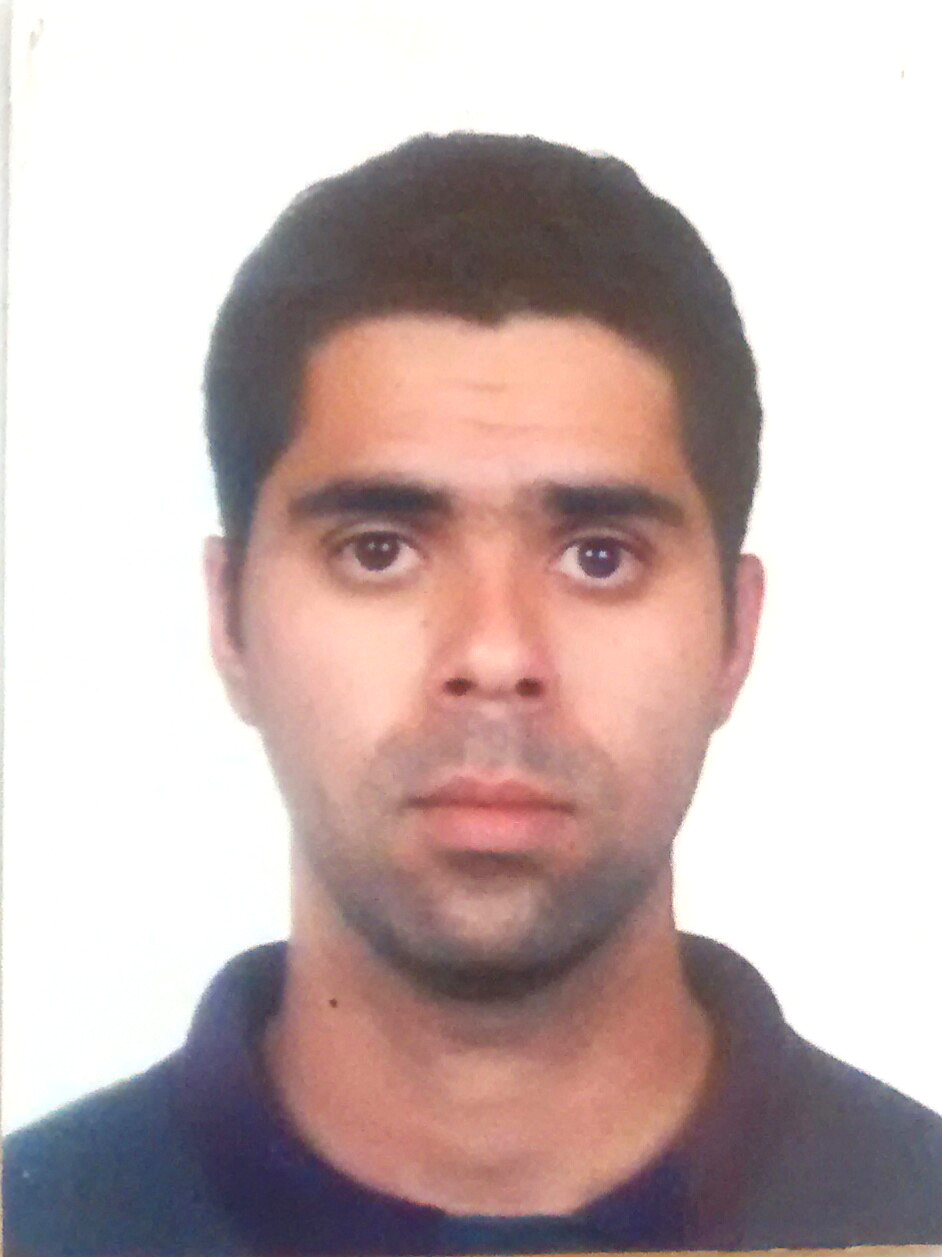
\includegraphics[width=2.0cm]{foto2.jpg}  } 	\\
Domicilio: Corregidora, Querétaro  	&  Celular: +52 443 155 5416	 		&	\\
		& 	Skype ID: rdglpz  			&	\\
%\\       		&	ORCID ID: 0000-0003-2772-0051						&
& & \\
\end{tabular}



\blankline

\blankline

\section{Empleo Actual}
Catedrático de tiempo completo, perteneciente al SNI (Nivel Candidato) del Consejo Nacional de Ciencia y Tecnología (CONACyT) comisionado en el consorcio CONACyT-CentroMet por medio del proyecto \textit{``Modelado espacio-temporal en y entre ciudades''} del Centro de Investigación en Geografía y Geomática Ing. Jorge L. Tamayo A.C. (CentroGeo).  \textit{(Desde el 1 de Noviembre del 2017)}. 
%\textbf{Actividad:} Catedrático Investigador en el proyecto "Modelaje espacio-temporal en y entre ciudades".


\blankline


\section{Intereses y Habilidades  } \textbf{Lenguajes de Programación y Manejadores de Bases de Datos}
 
Python R, Matlab Mathematica, Java, C/C++, PHP-HTML-MySQL(SQL), CassandraDB(NoSQL, Cassandra Query Language).

\blankline

\textbf{Investigación}
 
Aprendizaje automático (Máquinas de Vectores de Soporte, Redes Neuronales Artificiales, Lógica difusa), minería de datos (Algoritmos eficientes de búsqueda de vecinos cercanos), modelado y predicción de series de tiempo, predicción multimodelo con selección probabilista de modelos (Enfoque Bayesiano).
Heurísticas para Optimización global no convexa, análisis de estabilidad e identificación de parámetros de sistemas dinámicos no lineales.

 
\blankline

\section{Grupos de Investigación y Proyectos}
%Mexican Center of Energy Innovation Project.% Project: Forecasting the Natural Resources Required for the Production of Renewable Electric Power.
\textbf{Proyecto del Centro Mexicano de Innovación en Redes Eléctricas Inteligentes (CeMIE)}: Predicción de los recursos naturales requeridos para la producción de Energía eléctrica renovable. \url{https://www.ineel.mx/cemie.html}

%Applied Computational Intelligence Network.
\textbf{Grupo:} Red de Inteligencia Computacional Aplicada. \url{https://goo.gl/7B4RcE}. 
\blankline
 
\section{Idiomas} 
Inglés: 550 puntos TOEFL ITP. 

Italiano: Nivel B1 MCER. 


\section{Grado Académico}  \textbf{Ph.D in Computer Science and Engineering. Cédula pendiente}. (Con mención de \textit{Doctorado Europeo}).

\textbf{Institución}: Escuela de Estudios Avanzados de Lucca, Italia. \textit{(Feb-2012 Ene-2016)}. 

\textbf{Tesis:} Predicción de Series de Tiempo Basado en Clasificación de Patrones Dinámicos (Time Series Forecasting Based on Classification of Dynamic Patterns).

\textbf{Tutores:} Dr. Alberto Bemporad. Dr. Pantelis Sopasakis.

\textbf{Campo de estudio:} Estudio de series de tiempo.

\textbf{Materias cursadas:} Métodos formales y semántica. Complejidad de algoritmos, Álgebra lineal básica. Principios de programación paralela y concurrente. Modelado de desempeño aplicado a redes de computadoras. Modelado, especificación y verificación de sistemas reactivos. Introducción a optimización global y local. Análisis de desempeño con chequeo de modelos. Control óptimo (algoritmos de Optimización). Metodología de programación, \textit{Cloud Computing}. Teoría de Redes (Grafos) Complejas. Aprendizaje automático (Machine Learning). 

\blankline

\textbf{M.C. en Ingeniería Eléctrica (Grupo Sistemas Computacionales) Cédula: 6935145}.

\textbf{Institución}: Universidad Michoacana de San Nicolas de Hidalgo. Morelia, México. \textit{(Mar-2008 Ago-2010)}.

\textbf{Tesis:}  Diagramas de bifurcación para ecuaciones diferencial discontinuas o no diferenciables.

\textbf{Tutores:}  Dr. Juan Jose Flores Romero, Dr. Claudio Fuerte E.

%Campo de estudio:  Evolutionary computing, nonlinear dynamical systems, stability analysis and optimization.
\textbf{Campo de estudio:}  Computación evolutiva, análisis de estabilidad y optimización global no convexa de sistemas dinámicos no lineales.

\blankline

\textbf{Ingeniero en Sistemas Computacionales. Cédula: 5670139}.

\textbf{Institución}: Instituto Tecnológico de Morelia. Morelia, México. \textit{(2002 2007)}.

%Tesis: Implementation and performance analysis of \textbf{``Linux Terminal Server Project"} for educational purposes.
\textbf{Tesis:} Implementación y análisis de desempeño de ``Linux Terminal Server Project" para propósitos educativos.

\textbf{Campo de estudio:} Sistemas operativos distribuidos.

%\section{Academic Experience}  \textbf{Teaching}.
\section{Experiencia Académica}  \textbf{Enseñanza}.


\blankline
\textbf{Instituto Tecnológico de Morelia}. Morelia, México.

\begin{innerlist}
%\item Structured programming and object oriented programming (Electronic and  Industrial Engineering), Research Methodology (Computational Systems Engineering). \textit{(Aug-2011 Jan-2012)}.
\item Programación estructurada y programación orientada a objetos en Java y C++. (Ingeniería Industrial e Ingeniería Electrónica), Metodología de la Investigación (En Ingeniería en Sistemas Computacionales). \textit{(Ago-2011 Ene-2012)}.
%\item Database Fundamentals (Computational Systems Engineering), Structures and organization of data. (Technology Information Engineering) and Evaluation of software projects. \textit{(Jan-2011 Jul-2011)}.
\item Fundamentos de Base de Datos (Ingeniería en Sistemas Computacionales), Estructura y organización de datos en C. (Ingeniería en Tecnologías de la Información) y Evaluación de proyectos de software. \textit{(Ene-2011 Jul-2011)}.
%\item Operative systems, selected topics in programming and research fundamentals. \textit{(Aug-2010 Dec-2010)}.
\item Sistemas operativos, Tópicos Selectos de Programación, y Fundamentos de Investigación. \textit{(Ago-2010 Dic-2010)}.
\end{innerlist}


\blankline

\blankline
\textbf{Universidad de Morelia}. Morelia, México.

\begin{innerlist}
%\item Web programming with PHP. \textit{(Aug-2009 Dec-2009)}.
\item Programación web en PHP. \textit{(Ago-2009 Dic-2009)}.
\end{innerlist}

\blankline

%\section{Professional Experience}
\section{Experiencia Profesional}
%\subsection{Participation in Research Projects}
%\textbf{State Center for Information and Communications Technologies (CETIC)}. \textit{(Mar-2007 Jun-2007)}.




\textbf{Centro de Investigación y Estudios Avanzados del Instituto Politécnico Nacional (CINVESTAV-IPN)}. Ciudad de México. \textit{(Oct/2016 - Julio/2017)}

\textbf{Departamento de Coordinación y Gestión de Servicios de Tecnologías de Información y Comunicaciones (CGSTIC)}.

Desarrollo de agentes conversacionales inteligentes manejando gran volumen de información (Big Data) y Aprendizaje Automático (Machine Learning).


\blankline


\textbf{Universidad Michoacana de San Nicolás de Hidalgo: Centro de Cómputo y Procesos de Información Universitaria}. \textit{(Oct-2015  Oct-2016  )}.
Morelia, México

Programador y administrador de sistemas web y colaborador en la toma de decisiones relacionadas con el desarrollo de tecnología para la gestión eficiente de la información universitaria.

\blankline

\textbf{Centro Estatal de Tecnologías de la Información y Comunicaciones (CETIC)}. \textit{(Mar-2007 Jun-2007)}.
Morelia, México.

%Resident in physical infrastructure department.
Residente en el Departamento de Infraestructura Física.

%Project: Performance analysis of \textbf{Linux Terminal Server Project} applied to to basic education.
Proyecto: Análisis de desempeño de \textbf{Linux Terminal Server Project} aplicado a educación básica.

\blankline

{\textbf{Instituto Tecnológico de Morelia}}. Morelia, México. \textit{(Feb-2007)}

%Social Service Project: Develop of a PHP Web catalog for Social Service.
Proyecto servicio social: Desarrollo de un catálogo web de servicios sociales en PHP.

\blankline

%\textbf{IMPULSA}
%\blankline

%Participation in the young entrepreneurs program: IMPULSA.
%Participación en el programa de Jóvenes Emprendedores: IMPULSA

\blankline

\section{Publicaciones} \textbf{Artículos en Revistas Indexadas}
\blankline


\textbf{Aceptados en JCR}

%\subsection{Journal Articles Sent}
\begin{innerlist}

\item \textbf{Increasing weekend effect in ground-level O3 in metropolitan areas of Mexico} \textit{Iván Y. Hernández-Paniagua, Rodrigo Lopez-Farias, Jose J. Piña, Luis G. Ruíz-Suárez, Juan A. Pichardo-Corpus, Olivia Delgadillo, Agustín García-Reynoso, Arnoldo Flores-Torres, Alberto Mendoza}. {Sustainability}. (doi: 10.1109/ROPEC.2017.8261647) \textbf{Agosto 2018}.

\item \textbf{Multi-Model Prediction for Demand Forecast in
Water Distribution Networks} \textit{Rodrigo López Farías, Vicenc Puig, Héctor Rodriguez Rangel, Juan J. Flores} {Energies}. doi:10.3390/en11030660

\item  \textbf{Evolving Nearest Neighbor Time Series Forecasters.} \textit{Juan J. Flores, José Cede\~no Gonzalez, Rodrigo López Farías, Félix Calderón }.  {Journal of Soft Computing},
DOI : 10.1007/s00500-017-2822-1.
%\item \textit{Juan J. Flores, Rodrigo López Farías, Julio Barrera, Carlos Coello }.  Performance of Gravitational Interaction Optimization Metaheuristics on High Dimensional Problems.  Enviado a  \textit{Journal of Metaheuristics, \url{https://goo.gl/6bZ4tE}, el 1 de Febrero 2017}.

\item \textbf{Short-Term Demand Forecast using Bank of Neural Network Models Trained using Genetic Algorithms for the Optimal Management of Drinking Water Networks.}\textit{Hector Rodriguez Rangel, Vicen\c{c} Puig, Rodrigo López Farías, Juan J. Flores }.  {Journal of Hydroinformatics}. DOI: 10.2166/hydro.2016.199. ISSN: 1464-7141 \textbf{Noviembre 2016}.
%\item \textit{Juan J. Flores, Rodrigo López Farías, Julio Barrera, Carlos Coello }.  Performance of Gravitational Interaction Optimization Metaheuristics on High Dimensional Problems.  \textit{Journal of Metaheuristics}.(2016)
%\item \textit{Juan J. Flores, José Cede\~no Gonzalez, Rodrigo López Farías, Félix Calderón }.  Evolving Nearest Neighbor Time Series Forecasters. \textit{Journal of Time Series Analysis}.(2016)





\end{innerlist}

%\begin{innerlist}
%\item \textit{Juan J. Flores, José Cede\~no Gonzalez, Rodrigo López %Farías, Félix Calderón }.  Evolving Nearest Neighbor Time Series Forecasters. (Enviado a \textit{Journal of Soft Computing, \url{https://goo.gl/hSV5SV}}) Agosto 2017.
%\item \textit{Juan J. Flores, Rodrigo López Farías, Julio Barrera, Carlos Coello }.  Performance of Gravitational Interaction Optimization Metaheuristics on High Dimensional Problems.  Enviado a  \textit{Journal of Metaheuristics, \url{https://goo.gl/6bZ4tE}, el 1 de Febrero 2017}.
%\end{innerlist}


\textbf{Indexadas en otras revistas relevantes }
\begin{innerlist}
\item \textbf{Sistema de Medición de Flujos de Agua Tolerante a Fallos en Redes de Distribución de Agua Potable Utilizando Inteligencia Artificial}, \textit{H. Rodríguez Rangel, R. López Farías, G. Manjarrez Montelongo}, L. A. Morales Rosales y G. E. Peralta Peñuñuri. Komputer Sapiens, KS año 9 volumen 2, KS92, 2017, (Latin index).
\end{innerlist}



\blankline



\textbf{Artículos Aceptados en Conferencias Internacionales Arbitradas}

\blankline
%\textbf{Aceptados}
\begin{innerlist}

\item \textbf{Adaptive Nearest Neighbors Phase Space Reconstruction for Short-Time Prediction in Chaotic Time Series} \textit{Rodrigo López-Farías, José R. Cedeño Gonzalez, Olivia Delgadillo Ruiz, Juan J. Flores}. (ISBN-13: 9781941763957 ) .{The 10th International Multi-Conference on Complexity, Informatics and Cybernetics}, \textbf{Orlando, Estados Unidos, Marzo 2019}.


\item \textbf{Parameter Identification and Qualitative Analysis with Differential Evolution of the Calcium Standard Kinetics Model} \textit{Norma C. Perez-Rosas, Rodrigo López-Farías, Agustín Guerrero-Hernández and Juan J. Flores}. (DOI: 10.1109/ROPEC.2017.8261647) .{IEEE Autumn Meeting on Power, Electronics and Computing}, \textbf{Ixtapa México, Noviembre 2017}.


\item \textbf{Comparison of Time Series Forecasting Techniques with respect to Tolerance to Noise.} \textit{Juan J. Flores, Felix Calderon Solorio, Jose Rafael Cede\~no Gonzalez, Jose Ortiz Bejar and Rodrigo Lopez Farias}. (DOI: 10.1109/ROPEC.2016.7830618) .{IEEE Autumn Meeting on Power, Electronics and Computing}, \textbf{Ixtapa México, Noviembre 2016}.


\item \textbf{Holt-Winters Residual Modelling using an ANN trained by GA and Time Series Validation Applied to Water Demand Forecasting} \textit{Hector Rodriguez-Rangel, Vicen\c{c} Puig, Juan J. Flores and ,  Rodrigo López} Farías.. (Pendiente). {3rd International Conference on Control and Fault-Tolerant Systems} \textbf{Barcelona, España. Septiembre 2016}.

\item \textbf{Flow meter Data Validation and Reconstruction using Neural Networks: Application to the Barcelona Water Network} \textit{Hector Rodriguez Rangel, Vicen\c{c} Puig,Juan J. Flores and ,  Rodrigo López Farías.}. 2016 European Control Conference, Aalborg. Junio 2016. \url{https://goo.gl/i7muz7}. .

\item \textbf{Qualitative and Quantitative Mul} \textit{Rodrigo López Farías, Juan J. Flores and Vicen\c{c} Puig}.  ti-Model Forecasting with Nonlinear Noise Filter Applied to Water Demand \textit{IEEE Autumn Meeting on Power, Electronics and Computing}. DOI: 10.1109/ROPEC.2015.7395122.  \textbf{Ixtapa México, Noviembre 2015}.

\item \textbf{FNN a Fuzzy Version of the Nearest Neighbour Time Series Forecasting Technique } \textit{Juan J. Flores, Jose Ortiz Bejar, Jose Rafael Cedeño, Carlos Lara-Alvarez and Rodrigo López Farías}. {IEEE Autumn Meeting on Power, Electronics and Computing}. DOI: 10.1109/ROPEC.2015.7395125. \textbf{Ixtapa México, Noviembre 2015 }.

\item \textbf{A Multiple-Model Predictor Approach Based on an On-Line Mode Recognition with Application to Water Demand Forecasting} \textit{Rodrigo López Farías, Vicen\c{c} Puig}.  {International work-conference on Time Series 1. 
} URI https://goo.gl/njWQ1e. \textbf{Granada España, Julio 2015}.

\item \textbf{An implementation of a multi-model predictor based on the qualitative and quantitative decomposition of the time-series.} \textit{Rodrigo. López, Vicen\c{c} Puig, Hector Rodriguez.} URI http: //hdl.handle.net/2117/81862. {International work-conference on Time Series 1 
} \textbf{Granada España, Julio 2015}.

\item \textbf{Optimization with gravitational Interactions} \textit{Dr, Juan Flores, Rodrigo López, Julio Barrera.}   {ROPEC XIII: Autumn Meeting of Electric power systems, electronic and computation ( Reunión de Oto\~no de Potencia, Electrónica y Computación)} \textbf{ Morelia México, Noviembre 2011}.

\item \textbf{Gravitational Interactions Optimization.} Juan Flores, Rodrigo Lopez, Julio Barrera. {Learning and Intelligent OptimizatioN}  (LION 5) DOI 10.1007/978-3-642-25566-3\_17. \textbf{Roma, Italia - Enero 2011}. 

\item \textbf{Particle swarm optimization with gravitational interactions for multimodal and unimodal problems.} Juan J. Flores, Rodrigo Lopez and Julio Barrera.  In {Proceedings of the 9th Mexican International Conference on Artificial Intelligence (MICAI 2010)}, pages 3361-370. Springer-Verlag. DOI 10.1007/978-3-642-16773-7\_31. \textbf{Pachuca, México. Noviembre 2010.}

\end{innerlist}

\section{Conferencias, Seminarios y Talleres } \textbf{Impartido} \begin{innerlist}
 %\item Learning and Intelligent OptimizatioN - 'Gravitational Interactions Optimization'. (Roma, Italia. Enero 2011)
%\item IV National Seminar of computer learning and intelligence (SNAIC). Water demand prediction with Genetic Algorithms for the optimum optimization of a Drinking Water Distribution System. Instituto Nacional de Astrofísica, Óptica y Eléctrónica. Universidad Michoacana de San Nicolás de Hidalgo. (Morelia, México. Septiembre 2016).
\item 11$^o$ Congreso Estatal de Ciencia, Tecnología e Innovación, en  Ciencias de la Ingeniería y Tecnología. Búqueda del Clique con la mayor Interconectividad en un Grafo utilizando Optimización basado en Colonia de Hormigas. \textbf{Morelia, México. Octubre 2016}.

\item IV Seminario Nacional de Aprendizaje e Inteligencia Computacional (SNAIC). Predicción de la demanda de Agua con Algoritmos Genéticos para la optimización de la distribución de la Demanda de Agua en Redes de Agua Potable. Instituto Nacional de Astrofísica, Óptica y Electrónica. Universidad Michoacana de San Nicolás de Hidalgo. \textbf{Morelia, México. Septiembre 2016}..
 \item 10$^o$ Congreso Estatal de Ciencia, Tecnología e Innovación, en  Ciencias de la Ingeniería y Tecnología. PSO con Nichos Interactivos y B\'{u}squedas locales con Quasi-Newton. \textbf{Morelia, México. Septiembre 2015}.
 %\item Activities of X Anniversary of the Instituto Tecnológico Superior de Ciudad Hidalgo - ' Evolutionary computing applied to dynamical systems'.(Ciudad Hidalgo, México. October 2010).
 \item  Actividades del X aniversario del Instituto Tecnológico Superior de Ciudad Hidalgo. 'Evolutionary computing applied to dynamical systems'. \textbf{Ciudad Hidalgo, México. October 2010}.
%\item Week of Research Projects FIE of the UMSNH - 'Gravitational Interactions Optimization ' ( Morelia, México. Junio 2010 ).
\item Semana de Proyectos de Investigación de la Facultad de la UMSNH- 'Optimización con Interacciones Gravitacionales' \textbf{Morelia, México. Junio 2010}.
\item Semana de Proyectos de Investigación de la Facultad de la UMSNH - 'Diagramas de Bifurcación Utilizando Herramientas de Inteligencia Artificial' \textbf{Morelia, México. Junio 2009}.
\end{innerlist}

\blankline

\textbf{Atendido}
\begin{innerlist}
\item 5th HYCON2 Ph.D. School on Control of Networked and Large-Scale Systems and the EFFINET Ph.D. School on Control of Drinking Water Networks. \textbf{Lucca Italia, 1-5 de Julio 2013}
\item Taller de Java en la 2da semana de Computación y Sistemas Del Instituto Tecnológico Morelia. \textbf{Morelia, México. 2006.}
\item Análisis y Diseño Orientado a Objetos utilizando  UML  \textbf{Morelia México,  8-12 de Agosto 2011}

%\item Taller de Java en la 2da Semana de Sistemas y Computación (Morelia México, 2006)
%\item Week of Systems and computation in the Instituto Tecnológico de Morelia. \textit{Morelia, México (2006)}.
%\item 2da. Semana de Sistemas y Computaci\'on en el Instituto Tecnológico de Morelia (Morelia México, 2006).	
%\item Week of Systems and computation in the Instituto Tecnológico de Morelia. \textit{Morelia, México (2005).}
\end{innerlist}
%}



\end{document}




%%%%%%%%%%%%%%%%%%%%%%%%%% End CV Document %%%%%%%%%%%%%%%%%%%%%%%%%%%%%

%%%%%%%%%%%%%%%%%%%%%%%%%% Git Instructions %%%%%%%%%%%%%%%%%%%%%%%%%%%%
%cd /Users/rodrigolopez/rdglpzCV/rdglpzEngCV
%git add rdglpzCVEng.tex
%git add rdglpzCVEng.pdf
%git commit -m "Changes"
%git push origin master
%%%%%%%%%%%%%%%%%%%%%%%%%%%%%%%%%%%%%%%%%%%%%%%%%%%%%%%%%%%%%%%%%%%%%%%%%
